% Options for packages loaded elsewhere
\PassOptionsToPackage{unicode}{hyperref}
\PassOptionsToPackage{hyphens}{url}
\PassOptionsToPackage{dvipsnames,svgnames,x11names}{xcolor}
%
\documentclass[
  letterpaper,
  DIV=11,
  numbers=noendperiod]{scrartcl}

\usepackage{amsmath,amssymb}
\usepackage{iftex}
\ifPDFTeX
  \usepackage[T1]{fontenc}
  \usepackage[utf8]{inputenc}
  \usepackage{textcomp} % provide euro and other symbols
\else % if luatex or xetex
  \usepackage{unicode-math}
  \defaultfontfeatures{Scale=MatchLowercase}
  \defaultfontfeatures[\rmfamily]{Ligatures=TeX,Scale=1}
\fi
\usepackage{lmodern}
\ifPDFTeX\else  
    % xetex/luatex font selection
\fi
% Use upquote if available, for straight quotes in verbatim environments
\IfFileExists{upquote.sty}{\usepackage{upquote}}{}
\IfFileExists{microtype.sty}{% use microtype if available
  \usepackage[]{microtype}
  \UseMicrotypeSet[protrusion]{basicmath} % disable protrusion for tt fonts
}{}
\makeatletter
\@ifundefined{KOMAClassName}{% if non-KOMA class
  \IfFileExists{parskip.sty}{%
    \usepackage{parskip}
  }{% else
    \setlength{\parindent}{0pt}
    \setlength{\parskip}{6pt plus 2pt minus 1pt}}
}{% if KOMA class
  \KOMAoptions{parskip=half}}
\makeatother
\usepackage{xcolor}
\usepackage[left=1in,right=1in,top=1in,bottom=1in]{geometry}
\setlength{\emergencystretch}{3em} % prevent overfull lines
\setcounter{secnumdepth}{-\maxdimen} % remove section numbering
% Make \paragraph and \subparagraph free-standing
\makeatletter
\ifx\paragraph\undefined\else
  \let\oldparagraph\paragraph
  \renewcommand{\paragraph}{
    \@ifstar
      \xxxParagraphStar
      \xxxParagraphNoStar
  }
  \newcommand{\xxxParagraphStar}[1]{\oldparagraph*{#1}\mbox{}}
  \newcommand{\xxxParagraphNoStar}[1]{\oldparagraph{#1}\mbox{}}
\fi
\ifx\subparagraph\undefined\else
  \let\oldsubparagraph\subparagraph
  \renewcommand{\subparagraph}{
    \@ifstar
      \xxxSubParagraphStar
      \xxxSubParagraphNoStar
  }
  \newcommand{\xxxSubParagraphStar}[1]{\oldsubparagraph*{#1}\mbox{}}
  \newcommand{\xxxSubParagraphNoStar}[1]{\oldsubparagraph{#1}\mbox{}}
\fi
\makeatother

\usepackage{color}
\usepackage{fancyvrb}
\newcommand{\VerbBar}{|}
\newcommand{\VERB}{\Verb[commandchars=\\\{\}]}
\DefineVerbatimEnvironment{Highlighting}{Verbatim}{commandchars=\\\{\}}
% Add ',fontsize=\small' for more characters per line
\usepackage{framed}
\definecolor{shadecolor}{RGB}{241,243,245}
\newenvironment{Shaded}{\begin{snugshade}}{\end{snugshade}}
\newcommand{\AlertTok}[1]{\textcolor[rgb]{0.68,0.00,0.00}{#1}}
\newcommand{\AnnotationTok}[1]{\textcolor[rgb]{0.37,0.37,0.37}{#1}}
\newcommand{\AttributeTok}[1]{\textcolor[rgb]{0.40,0.45,0.13}{#1}}
\newcommand{\BaseNTok}[1]{\textcolor[rgb]{0.68,0.00,0.00}{#1}}
\newcommand{\BuiltInTok}[1]{\textcolor[rgb]{0.00,0.23,0.31}{#1}}
\newcommand{\CharTok}[1]{\textcolor[rgb]{0.13,0.47,0.30}{#1}}
\newcommand{\CommentTok}[1]{\textcolor[rgb]{0.37,0.37,0.37}{#1}}
\newcommand{\CommentVarTok}[1]{\textcolor[rgb]{0.37,0.37,0.37}{\textit{#1}}}
\newcommand{\ConstantTok}[1]{\textcolor[rgb]{0.56,0.35,0.01}{#1}}
\newcommand{\ControlFlowTok}[1]{\textcolor[rgb]{0.00,0.23,0.31}{\textbf{#1}}}
\newcommand{\DataTypeTok}[1]{\textcolor[rgb]{0.68,0.00,0.00}{#1}}
\newcommand{\DecValTok}[1]{\textcolor[rgb]{0.68,0.00,0.00}{#1}}
\newcommand{\DocumentationTok}[1]{\textcolor[rgb]{0.37,0.37,0.37}{\textit{#1}}}
\newcommand{\ErrorTok}[1]{\textcolor[rgb]{0.68,0.00,0.00}{#1}}
\newcommand{\ExtensionTok}[1]{\textcolor[rgb]{0.00,0.23,0.31}{#1}}
\newcommand{\FloatTok}[1]{\textcolor[rgb]{0.68,0.00,0.00}{#1}}
\newcommand{\FunctionTok}[1]{\textcolor[rgb]{0.28,0.35,0.67}{#1}}
\newcommand{\ImportTok}[1]{\textcolor[rgb]{0.00,0.46,0.62}{#1}}
\newcommand{\InformationTok}[1]{\textcolor[rgb]{0.37,0.37,0.37}{#1}}
\newcommand{\KeywordTok}[1]{\textcolor[rgb]{0.00,0.23,0.31}{\textbf{#1}}}
\newcommand{\NormalTok}[1]{\textcolor[rgb]{0.00,0.23,0.31}{#1}}
\newcommand{\OperatorTok}[1]{\textcolor[rgb]{0.37,0.37,0.37}{#1}}
\newcommand{\OtherTok}[1]{\textcolor[rgb]{0.00,0.23,0.31}{#1}}
\newcommand{\PreprocessorTok}[1]{\textcolor[rgb]{0.68,0.00,0.00}{#1}}
\newcommand{\RegionMarkerTok}[1]{\textcolor[rgb]{0.00,0.23,0.31}{#1}}
\newcommand{\SpecialCharTok}[1]{\textcolor[rgb]{0.37,0.37,0.37}{#1}}
\newcommand{\SpecialStringTok}[1]{\textcolor[rgb]{0.13,0.47,0.30}{#1}}
\newcommand{\StringTok}[1]{\textcolor[rgb]{0.13,0.47,0.30}{#1}}
\newcommand{\VariableTok}[1]{\textcolor[rgb]{0.07,0.07,0.07}{#1}}
\newcommand{\VerbatimStringTok}[1]{\textcolor[rgb]{0.13,0.47,0.30}{#1}}
\newcommand{\WarningTok}[1]{\textcolor[rgb]{0.37,0.37,0.37}{\textit{#1}}}

\providecommand{\tightlist}{%
  \setlength{\itemsep}{0pt}\setlength{\parskip}{0pt}}\usepackage{longtable,booktabs,array}
\usepackage{calc} % for calculating minipage widths
% Correct order of tables after \paragraph or \subparagraph
\usepackage{etoolbox}
\makeatletter
\patchcmd\longtable{\par}{\if@noskipsec\mbox{}\fi\par}{}{}
\makeatother
% Allow footnotes in longtable head/foot
\IfFileExists{footnotehyper.sty}{\usepackage{footnotehyper}}{\usepackage{footnote}}
\makesavenoteenv{longtable}
\usepackage{graphicx}
\makeatletter
\def\maxwidth{\ifdim\Gin@nat@width>\linewidth\linewidth\else\Gin@nat@width\fi}
\def\maxheight{\ifdim\Gin@nat@height>\textheight\textheight\else\Gin@nat@height\fi}
\makeatother
% Scale images if necessary, so that they will not overflow the page
% margins by default, and it is still possible to overwrite the defaults
% using explicit options in \includegraphics[width, height, ...]{}
\setkeys{Gin}{width=\maxwidth,height=\maxheight,keepaspectratio}
% Set default figure placement to htbp
\makeatletter
\def\fps@figure{htbp}
\makeatother

\usepackage{booktabs}
\usepackage{longtable}
\usepackage{array}
\usepackage{multirow}
\usepackage{wrapfig}
\usepackage{float}
\usepackage{colortbl}
\usepackage{pdflscape}
\usepackage{tabu}
\usepackage{threeparttable}
\usepackage{threeparttablex}
\usepackage[normalem]{ulem}
\usepackage{makecell}
\usepackage{xcolor}
\usepackage{fvextra}
\DefineVerbatimEnvironment{Highlighting}{Verbatim}{breaklines,commandchars=\\\{\}}
\DefineVerbatimEnvironment{OutputCode}{Verbatim}{breaklines,commandchars=\\\{\}}
\KOMAoption{captions}{tableheading}
\makeatletter
\@ifpackageloaded{caption}{}{\usepackage{caption}}
\AtBeginDocument{%
\ifdefined\contentsname
  \renewcommand*\contentsname{Table of contents}
\else
  \newcommand\contentsname{Table of contents}
\fi
\ifdefined\listfigurename
  \renewcommand*\listfigurename{List of Figures}
\else
  \newcommand\listfigurename{List of Figures}
\fi
\ifdefined\listtablename
  \renewcommand*\listtablename{List of Tables}
\else
  \newcommand\listtablename{List of Tables}
\fi
\ifdefined\figurename
  \renewcommand*\figurename{Figure}
\else
  \newcommand\figurename{Figure}
\fi
\ifdefined\tablename
  \renewcommand*\tablename{Table}
\else
  \newcommand\tablename{Table}
\fi
}
\@ifpackageloaded{float}{}{\usepackage{float}}
\floatstyle{ruled}
\@ifundefined{c@chapter}{\newfloat{codelisting}{h}{lop}}{\newfloat{codelisting}{h}{lop}[chapter]}
\floatname{codelisting}{Listing}
\newcommand*\listoflistings{\listof{codelisting}{List of Listings}}
\makeatother
\makeatletter
\makeatother
\makeatletter
\@ifpackageloaded{caption}{}{\usepackage{caption}}
\@ifpackageloaded{subcaption}{}{\usepackage{subcaption}}
\makeatother

\ifLuaTeX
  \usepackage{selnolig}  % disable illegal ligatures
\fi
\usepackage{bookmark}

\IfFileExists{xurl.sty}{\usepackage{xurl}}{} % add URL line breaks if available
\urlstyle{same} % disable monospaced font for URLs
\hypersetup{
  pdftitle={Case Study 1: Your Informative Title Here},
  pdfauthor={Miya Dang, Mia Tran},
  colorlinks=true,
  linkcolor={blue},
  filecolor={Maroon},
  citecolor={Blue},
  urlcolor={Blue},
  pdfcreator={LaTeX via pandoc}}


\title{Case Study 1: Your Informative Title Here}
\author{Miya Dang, Mia Tran}
\date{2025-03-05}

\begin{document}
\maketitle


\emph{Your written short report should be the first thing your reader
encounters in your case study document. While you may choose to label
each of the required components/sections of the short report with its
own header (see below for an example of creating a header in Quarto),
you do not need to do so provided that all of the required information
is included. Your report should be self-contained and written in such a
way that a quantitatively inclined friend (who has taken or is taking
SDS 291) could follow what you did without necessarily knowing anything
about the U.S. presidential election of 2000.}

\emph{As you write your report, you may wish to reference the guide to
typesetting regression lines in Quarto using LaTeX (linked at the top of
our class Moodle page), the Quarto help page for formatting documents
using Markdown (https://quarto.org/docs/authoring/markdown-basics.html),
and the Quarto help page for customizing the output from executed code
chunks (https://quarto.org/docs/computations/execution-options.html).}

\subsubsection{An example section
heading}\label{an-example-section-heading}

\emph{When you create plots for your case study report, the
\texttt{echo:\ false} chunk option tells Quarto to include the final
output of your R commands (in this case, a plot) in your rendered PDF
\emph{without} printing the underlying R commands that generated that
plot! The message and warning flags both prevent R from printing any
additional text with error messages or warnings to the PDF.}

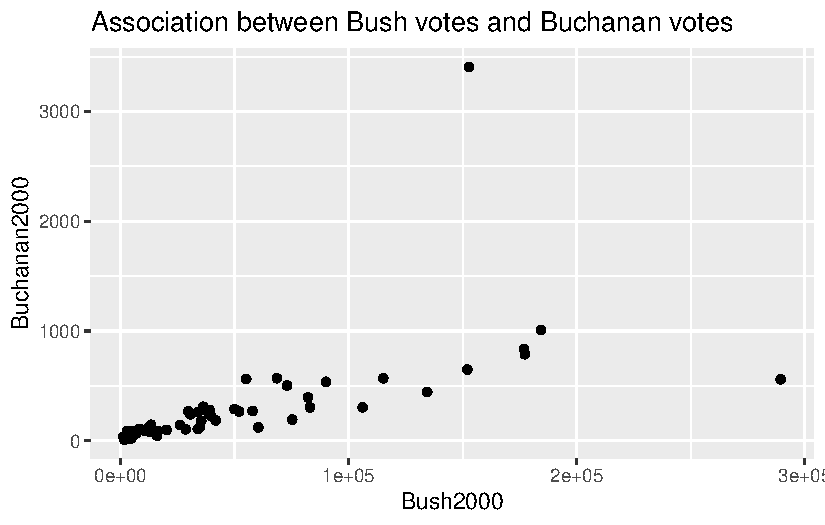
\includegraphics{SDS-291-case-study-1_files/figure-pdf/unnamed-chunk-2-1.pdf}

\emph{When reporting the results of your regression analysis, I would
like you to write out a mathematical description of the main/final
population model for the mean. Here is an example of what that might
look like:}

Let \(mort_i\) denote the heart disease mortality rate in country \(i\)
(measured in deaths per 1,000 individuals) and \(wine_i\) denote the
consumption of wine (measured in liters per person per year). Our final
linear regression model is
\[E[mort_i | wine_i] = \beta_0 + \beta_1\left(wine_i\right).\]

\emph{You do not need to write out the fitted regression line, but you
should (at a minimum) provide a table summarizing the estimated
coefficients of the model and their corresponding standard errors, like
the one shown below. A print-out from the \texttt{summary()} command
alone is not sufficient.}

\begin{table}[H]
\centering
\begin{tabular}[t]{lcccc}
\toprule
  & Name for Col. 1 & Name for Col. 2 & Name for Col. 3 & Name for Col. 4\\
\midrule
(Intercept) & 7.69 & 0.47 & 16.24 & 0e+00\\
Wine & -0.08 & 0.02 & -4.48 & 4e-04\\
\bottomrule
\end{tabular}
\end{table}

\section{R Appendix}\label{r-appendix}

\emph{Copy and paste all code that you used for your case study into one
chunk at the end of your written report. Before submitting your case
study, take one final look at the R Appendix and make sure that all code
is clearly visible. If you see a line running off the side of the PDF,
please split the code over multiple lines using a linebreak. The header
at the top of this template should ensure that lines of code are
automatically wrapped in your final document.}

\begin{Shaded}
\begin{Highlighting}[]
\CommentTok{\# Loading necessary packages}
\FunctionTok{library}\NormalTok{(tidyverse)}
\FunctionTok{library}\NormalTok{(Sleuth2)}
\FunctionTok{library}\NormalTok{(broom)        }
\FunctionTok{library}\NormalTok{(kableExtra)   }

\CommentTok{\# Loading the data for case study one}
\NormalTok{election }\OtherTok{\textless{}{-}}\NormalTok{ Sleuth2}\SpecialCharTok{::}\NormalTok{ex0825}

\CommentTok{\# Creating a second dataset with Palm Beach County excluded}
\NormalTok{election\_wo\_pb }\OtherTok{\textless{}{-}}\NormalTok{ election }\SpecialCharTok{|\textgreater{}} \FunctionTok{filter}\NormalTok{(County }\SpecialCharTok{!=} \StringTok{"Palm Beach"}\NormalTok{)}

\CommentTok{\# Loading another dataset on wine consumption and heart disease mortality}
\NormalTok{wine }\OtherTok{\textless{}{-}}\NormalTok{ Sleuth2}\SpecialCharTok{::}\NormalTok{ex0823}

\CommentTok{\# Creating a scatterplot for the relationship between mortality and wine consumption}
\NormalTok{wine }\SpecialCharTok{|\textgreater{}} \FunctionTok{ggplot}\NormalTok{(}\FunctionTok{aes}\NormalTok{(}\AttributeTok{x =}\NormalTok{ Wine, }\AttributeTok{y =}\NormalTok{ Mortality)) }\SpecialCharTok{+} \FunctionTok{geom\_point}\NormalTok{() }\SpecialCharTok{+} 
  \FunctionTok{ggtitle}\NormalTok{(}\StringTok{"Association between wine consumption and mortality rates."}\NormalTok{)}
\end{Highlighting}
\end{Shaded}

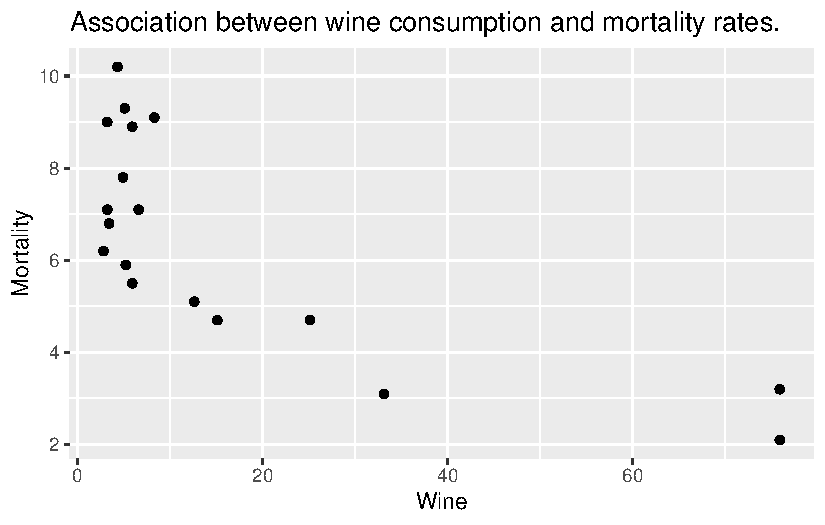
\includegraphics{SDS-291-case-study-1_files/figure-pdf/unnamed-chunk-4-1.pdf}

\begin{Shaded}
\begin{Highlighting}[]
\CommentTok{\# Fitting and summarizing the regression line for mean mortality }
\CommentTok{\# as a function of wine consumption}
\NormalTok{wine.lm }\OtherTok{\textless{}{-}} \FunctionTok{lm}\NormalTok{(Mortality }\SpecialCharTok{\textasciitilde{}}\NormalTok{ Wine, }\AttributeTok{data =}\NormalTok{ wine)}
\NormalTok{wine.lm.table }\OtherTok{\textless{}{-}}\NormalTok{ wine.lm }\SpecialCharTok{|\textgreater{}} \FunctionTok{tidy}\NormalTok{()}
\NormalTok{wine.lm.table }\SpecialCharTok{|\textgreater{}} \FunctionTok{kbl}\NormalTok{(}\AttributeTok{col.names =} \FunctionTok{c}\NormalTok{(}\StringTok{"Name for Col. 1"}\NormalTok{, }\StringTok{"Name for Col. 2"}\NormalTok{, }
                                   \StringTok{"Name for Col. 3"}\NormalTok{, }\StringTok{"Name for Col. 4"}\NormalTok{, }
                                   \StringTok{"Name for Col. 5"}\NormalTok{), }
                     \AttributeTok{align =} \StringTok{"c"}\NormalTok{, }\AttributeTok{booktabs =}\NormalTok{ T, }\AttributeTok{linesep=}\StringTok{""}\NormalTok{, }
                     \AttributeTok{digits =} \FunctionTok{c}\NormalTok{(}\DecValTok{2}\NormalTok{, }\DecValTok{2}\NormalTok{, }\DecValTok{2}\NormalTok{, }\DecValTok{4}\NormalTok{)) }\SpecialCharTok{|\textgreater{}} 
  \FunctionTok{kable\_classic}\NormalTok{(}\AttributeTok{full\_width =}\NormalTok{ F, }\AttributeTok{latex\_options =} \FunctionTok{c}\NormalTok{(}\StringTok{"HOLD\_position"}\NormalTok{))}
\end{Highlighting}
\end{Shaded}

\begin{table}[H]
\centering
\begin{tabular}[t]{ccccc}
\toprule
Name for Col. 1 & Name for Col. 2 & Name for Col. 3 & Name for Col. 4 & Name for Col. 5\\
\midrule
(Intercept) & 7.69 & 0.47 & 16.2396 & 0\\
Wine & -0.08 & 0.02 & -4.4750 & 0\\
\bottomrule
\end{tabular}
\end{table}




\end{document}
